A continuación, se presentan los resultados obtenidos en la validación del sistema Thary. Estos resultados se obtuvieron luego de aplicar la estrategia de validación ya definida anteriormente, sobre el historial real de consumo de 856 productos (medicamentos) del año 2021 - 2022 en la Clínica Nuestra Señora de los remedios. 

Las métricas obtenidas al evaluar los tres modelos candidatos, junto con el método de selección de modelo por producto. Todo esto sobre el último periodo de prueba disponible, que corresponde al trimestre abril-junio de 2022, con seis meses de entrenamiento previo.

\begin{table}[H]
    \centering
    \caption{Métricas del holdout final por modelo.}
    \label{tab:resultados_holdout}
    \renewcommand{\arraystretch}{1.3}
    \begin{tabularx}{\textwidth}{|X|c|c|c|c|c|}
    \hline
    \textbf{Modelo} & \textbf{MAE} & \textbf{RMSE} & \textbf{Mediana Error} & \textbf{MAPE (\%)} & \textbf{WAPE (\%)} \\
    \hline
    Media Móvil (3 meses) & 48.79 & 243.65 & 5.33 & 80.32 & 23.86 \\
    \hline
    Regresión Lineal      & 56.43 & 276.41 & 5.25 & 95.30 & 27.60 \\
    \hline
    XGBoost (log1p)       & 50.59 & 254.82 & 3.53 & 65.12 & 24.74 \\
    \hline
    \textbf{Sistema final (selección por producto)} & \textbf{48.47} & \textbf{243.55} & --- & \textbf{79.33} & \textbf{23.71} \\
    \hline
    \end{tabularx}
\end{table}

\begin{figure}[H]
    \centering
    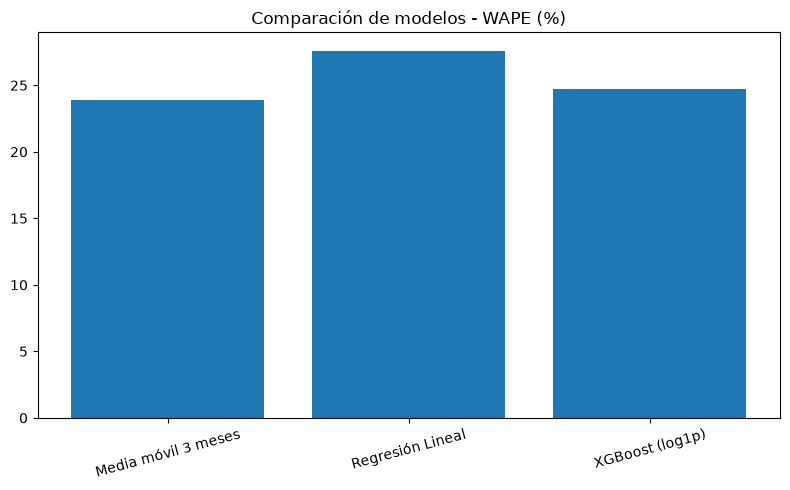
\includegraphics[width=0.75\textwidth]{templatefigures/comparacion_WAPE_porcentaje}
    \caption{Comparación de WAPE entre los tres modelos candidatos (holdout final).}
    \label{fig:comparacion_wape}
\end{figure}

\subsubsection{Consistencia mediante validación cruzada temporal}

Después de obtener los resultados anteriores, se propuso el uso de una validación cruzada para descartar que el resultado obtenido dependiera de las condiciones y particularidades de un único periodo de prueba.

La idea principal, es probar el modelo varias veces simulando estar en un mes distinto al pasado, para poder evaluar si acierta de forma consistente y no solo una vez por casualidad. Para poder predecir un mes, solo se puede usar los meses que vinieron antes, no se pueden usar los datos que serían "Futuros", porque queremos simular un escenario real, y en ese caso, no se tendría esa información.

\begin{enumerate}
    \item Prueba 1 (Fold 1): Es el más antiguo, se le enseña al modelo con los 4 meses previos a febrero de 2022, y se hace que el sistema adivine febrero, marzo y abril de 2022. Se compara lo que adivino contra los resultados reales de esos meses y se registra que tan grande fue el error.
    \item Prueba 2 (Fold 2): En esta segunda prueba o Fold, se le enseña al modelo con 5 meses en vez de 4, es decir, los meses previos a marzo de 2022, y se le pide que prediga marzo, abril y mayo de 2022, una vez más, se compara y se registra el error.
    \item Prueba 3 (Fold 3): Por último, se le enseña al modelo con los 6 meses previos a abril de 2022 y se le solicita al sistema que prediga abril, mayo y junio de 2022, se compara y, una vez más, se registra el error. Este último fold corresponde al mismo holdout final presentado en la Tabla \ref{tab:resultados_holdout}.
\end{enumerate}


Dicha validación cruzada temporal se implementó en el sistema en el archivo \texttt{app/services/prediccion/validacion.py}.

\Needspace{10\baselineskip}
\captionof{listing}{Constantes y función \texttt{\_armar\_folds} de la validación cruzada temporal.}\label{lst:validacion_folds}
\begin{minted}{python}
TEST_SIZE_MESES = 3
MIN_TRAIN_MESES = 3
MAX_FOLDS = 3


def _armar_folds(meses_ordenados):
    n = len(meses_ordenados)
    folds = []
    fin_test = n
    while len(folds) < MAX_FOLDS:
        inicio_test = fin_test - TEST_SIZE_MESES
        if inicio_test < MIN_TRAIN_MESES:
            break
        folds.append((meses_ordenados[:inicio_test], meses_ordenados[inicio_test:fin_test]))
        fin_test -= 1
    folds.reverse()
    return folds
\end{minted}

Se definen tres constantes, \texttt{TEST\_SIZE\_MESES}, \texttt{MIN\_TRAIN\_MESES} y \texttt{MAX\_FOLDS}, que definen el tamaño de la ventana de prueba, el tamaño mínimo de la ventana de entrenamiento y el número máximo de folds a generar, respectivamente.


Se arma la función que genera las particiones \texttt{\_armar\_folds}, esta recibe una lista de todos los meses disponibles organizados cronologicamente. Se define el fold más reciente, es decir, los últimos meses disponibles \texttt{TEST\_SIZE\_MESES}. En cada iteracion se retrocede el punto de corte de un mes hacia atrás en el tiempo, de esta manera, se crea un nuevo Fold cuyo entrenamiento crece en un mes respecto al anterior. Este proceso se repite hasta completar \texttt{MAX\_FOLDS}, o hasta que ya no quede suficiente historial y el tamaño de la ventana de entrenamiento sea menor a \texttt{MIN\_TRAIN\_MESES} meses de entrenamiento.  

Al finalizar, los folds se ordenan en orden cronológico del más antiguo al más nuevo antes de ser devueltos.

Al ya tener los folds organizados, el sistema entrena nuevamente los tres modelos candidatos, y selecciona el mejor modelo por producto, evaluando el resultado bajo la etiqueta de "Sistema final". Es decir, es la estrategia que usa Thary para predecir el consumo, en vez de escoger uno solo, para cada producto, el sistema entrena los 3 modelos y selecciona el que se equivocó menos con ese producto en particular.

Un aspecto importante es que, la elección de qué modelo usar para cada producto se hace solo con los datos de entrenamiento, antes de ver los datos de prueba. Esto demuestra que no se está "haciendo trampa", ya que el sistema no tiene acceso a los datos de prueba, y por lo tanto, no puede "aprender" de ellos.

Aun así, solo esto no basta para confiar en el resultado, ya que aun si el sistema está eligiendo el modelo de forma honesta, un único experimento podría haber salido bien por casualidad y no porque el sistema de verdad sea bueno.


Es por eso que la validación cruzada aportó valor al sistema, ya que al repetir este mismo proceso (entrenamiento, elección del modelo y evaluación) en diferentes periodos de prueba, se confirma que el resultado obtenido en el holdout final no fue un resultado aislado, sino que se repite de forma consistente en distintos periodos de prueba.

En la siguiente tabla se describen el promedio y la desviación estándar de las métricas obtenidas en cada fold, para cada modelo candidato y el sistema final:

\begin{table}[H]
    \centering
    \caption{Resumen de la validación cruzada temporal (promedio $\pm$ desviación, 3 folds).}
    \label{tab:resumen_cv}
    \renewcommand{\arraystretch}{1.3}
    \begin{tabularx}{\textwidth}{|X|c|c|c|c|}
    \hline
    \textbf{Modelo} & \textbf{MAE} & \textbf{RMSE} & \textbf{MAPE (\%)} & \textbf{WAPE (\%)} \\
    \hline
    Media Móvil        & 44.27 $\pm$ 3.70  & 200.82 $\pm$ 41.31 & 82.38 $\pm$ 1.85  & 22.31 $\pm$ 1.29 \\
    \hline
    Regresión Lineal   & 58.13 $\pm$ 2.21  & 270.35 $\pm$ 6.32  & 106.24 $\pm$ 10.64 & 29.38 $\pm$ 1.84 \\
    \hline
    XGBoost            & 46.58 $\pm$ 3.46  & 223.64 $\pm$ 31.40 & 64.93 $\pm$ 2.25  & 23.48 $\pm$ 1.15 \\
    \hline
    \textbf{Sistema final} & \textbf{43.42 $\pm$ 3.77} & \textbf{190.50 $\pm$ 40.63} & \textbf{81.13 $\pm$ 1.56} & \textbf{21.88 $\pm$ 1.34} \\
    \hline
    \end{tabularx}
\end{table}

De la tabla se puede observar que:

\begin{itemize}
    \item El sistema final es el que obtiene el mejor promedio en las cuatro
    métricas evaluadas. En cuanto a la estabilidad entre folds, presenta la
    menor desviación estándar en RMSE y MAPE, aunque una desviación ligeramente
    mayor a la de la Media Móvil en MAE y WAPE. Esto es significativo, porque
    demuestra que vale la pena la complejidad de elegir un modelo distinto para
    cada producto: el sistema final es consistentemente más preciso en promedio,
    aunque su ventaja en estabilidad no se cumple de forma uniforme en las
    cuatro métricas.
    \item La media móvil es el segundo mejor modelo, seguido por XGBoost y finalmente la regresión lineal. Cuando se comparan los tres modelos candidatos de forma individual, la media móvil es la que obtiene un mejor MAE, RMSE y WAPE, mientras que solo XGBoost la supera en MAPE. El hecho de que ninguno de los dos modelos más sofisticados domine de forma general sobre la línea base avala la decisión de seleccionar un modelo distinto por producto, ya que no existe un único modelo que sea el mejor en todos los casos.
    \item La Regresión Lineal es la que tiene los peores resultados en las cuatro métricas, además de que su MAPE es el que más varía entre los 3 folds. Esto es coherente con la tendencia de este modelo a sobreestimar los productos de alta demanda, observada previamente en el análisis de dispersión entre modelos, lo que ayuda a explicar por que su error resulta más alto que el de los otros dos modelos.
    \item Finalmente, se observa que la efectividad del sistema final no se debe solamente a "elegir el mejor modelo en general", que en este caso seria la media móvil, sino a elegir un modelo distinto para cada producto. En caso de haber elegido media móvil para todos los productos, el error hubiera sido de 22.31\% de WAPE, mientras que al elegir el mejor modelo por producto, validado mediante la prueba de Diebold-Mariano, el error se reduce a 21.88\%
\end{itemize}